Background subtraction in \texttt{CalibrateImageTask} estimates and removes large-scale background signals from science imaging prior to source detection and measurement.
Such signals include sky brightness from airglow, moonlight, scattered light, zodiacal light, and diffuse astrophysical emission.
The background is estimated twice: an initial model (\texttt{psf\_subtract\_background}) is subtracted before PSF characterization, and a second model (\texttt{star\_background}) is fit on the updated source-masked image before the final detection pass.
Each post-ISR image is divided into $128 \times 128$\,pixel superpixels, and the iterative $3\sigma$-clipped mean of unmasked pixels in each bin is fit with a sixth-order two-dimensional Chebyshev polynomial, evaluated at native pixel resolution via Akima spline interpolation.
Before fitting \texttt{star\_background}, the \texttt{DETECTED} mask plane is dilated by up to 10\,pixels to suppress source-wing flux from leaking into background bins.
After \texttt{star\_background} subtraction, a zeroth-order pedestal correction is estimated iteratively over bin sizes starting at $32 \times 32$\,pixels, doubling each step until the cumulative pedestal level changes by less than 5\% or 0.5\,counts between steps.
The \texttt{star\_background} model and pedestal corrections together constitute the output background model (\texttt{preliminary\_visit\_image\_background}; see Figure~\ref{fig:background-example}).

\begin{figure*}
    \centering
    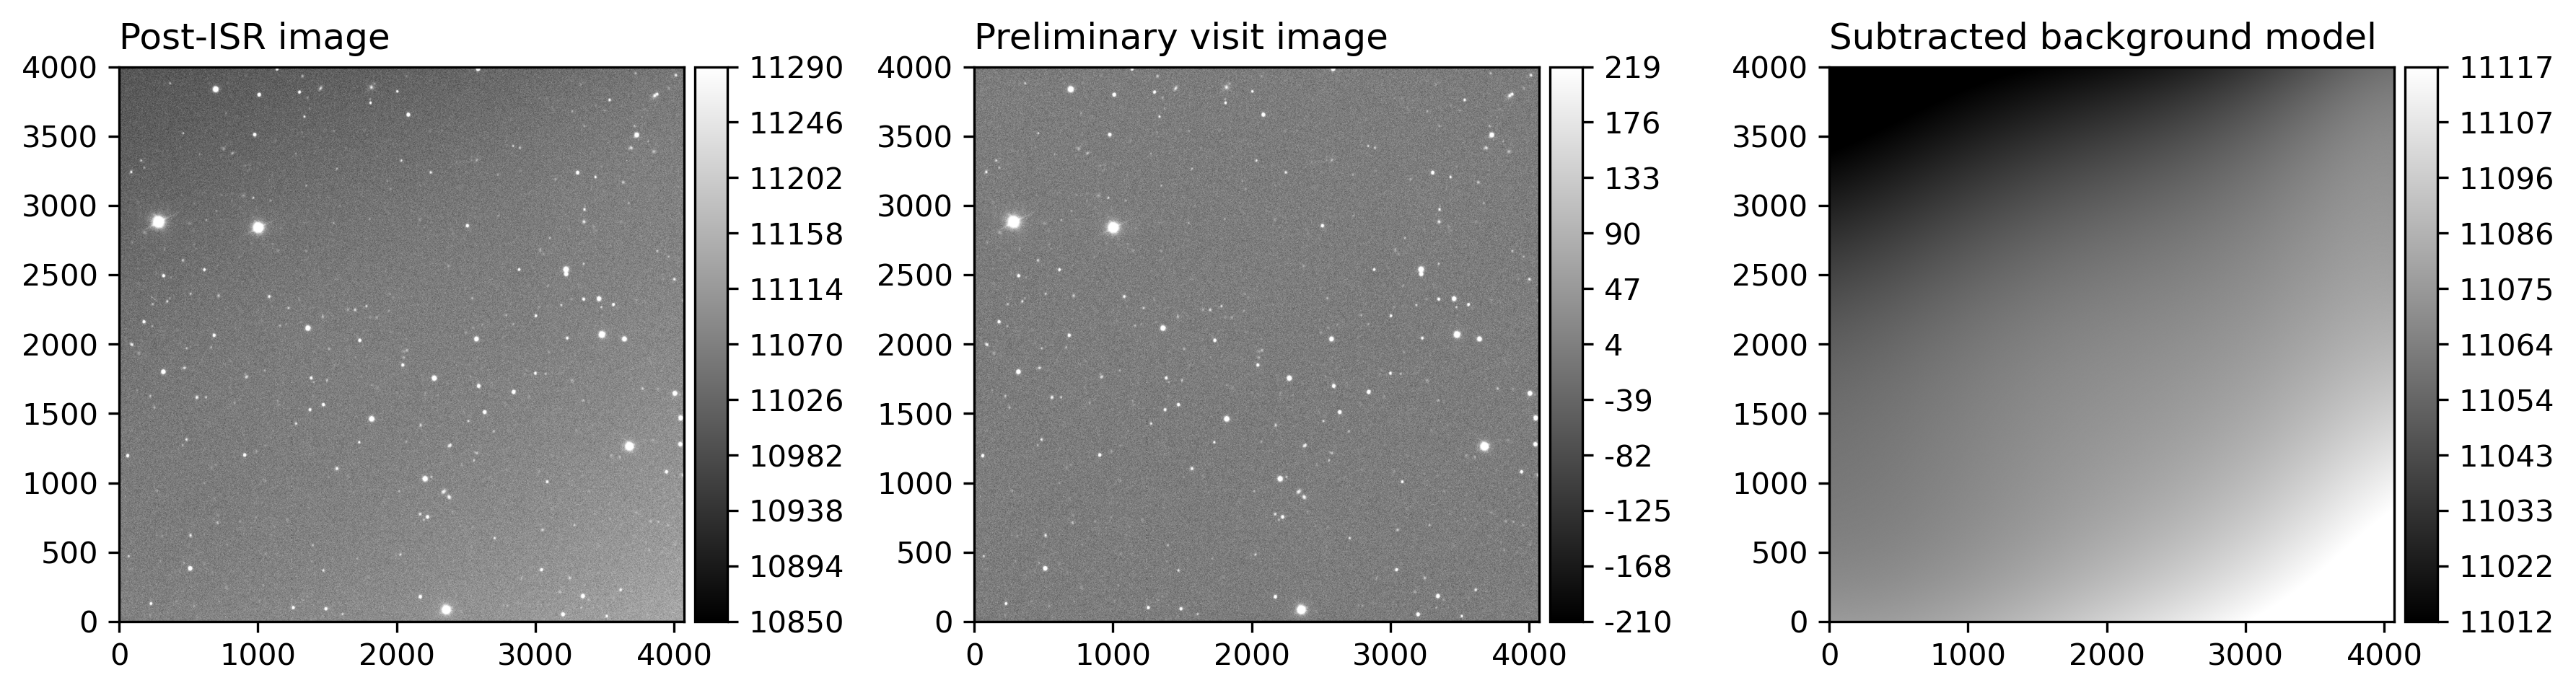
\includegraphics[width=\textwidth]{figures/background_visit2025110500300_det025}
    \caption{
        Background subtraction for LSSTCam visit~2025110500300, detector~25.
        \textit{Left:} Post-ISR image (\texttt{post\_isr\_image}), before any background removal.
        \textit{Center:} Preliminary visit image (\texttt{preliminary\_visit\_image}), after background subtraction by \texttt{CalibrateImageTask}.
        \textit{Right:} The subtracted background model (\texttt{preliminary\_visit\_image\_background}), illustrating the large-scale structure removed.
        All three panels use a linear stretch clipped to the central 95th percentile of pixel values.
    }
    \label{fig:background-example}
\end{figure*}

Compared to DP1~\citep{dp1}, several changes were made to background subtraction for DP2\@.
The inline re-estimation performed after each detection pass in DP1 (\texttt{reEstimateBackground = True}) has been replaced by the dedicated \texttt{star\_background} subtask.
In addition to source mask dilation and a pedestal correction, other new features for DP2 include adaptive threshold determination and diffraction spike masking.
The per-step illumination correction used in DP1 has been disabled for DP2.
Following background subtraction, the median and standard deviation of all unmasked pixels and of \textit{sky source} fluxes are recorded in the task metadata as diagnostics of background subtraction quality.
